\documentclass[12pt, twoside]{article}
\usepackage[letterpaper, margin=1in, head=30pt, headsep=0.1in]{geometry}
\usepackage[english]{babel}
\usepackage[utf8]{inputenc}
\usepackage{amsmath}
\usepackage{amsfonts}
\usepackage{amssymb}
\usepackage{tikz}
%\usetikzlibrary{quotes, angles}

\usepackage{graphicx}
\usepackage{enumitem}
\usepackage{multicol}

\newif\ifmeta
\metatrue %print standards and topics tags

\title{Regents Geometry}
\author{Chris Huson}
\date{October 2021}

\usepackage{fancyhdr}
\pagestyle{fancy}
\fancyhf{}
\renewcommand{\headrulewidth}{0pt} % disable the underline of the header
\raggedbottom


\fancyhead[LE]{\thepage}
\fancyhead[RO]{\thepage \\ Name: \hspace{4cm} \,\\}
\fancyhead[LO]{BECA / Dr. Huson / IB Math 6 Geometry}

\begin{document}
\subsubsection*{6.10: Applying Algebra to Geometric Situations}
\begin{enumerate}
\item Write down the slope perpendicular to the given slope. \vspace{0.5cm}
  \begin{enumerate}
    \begin{multicols}{2}
    \item   $m= -\frac{4}{3} \hspace{1cm} m_{\perp} = $ \vspace{1cm}
    \item   $m= 3 \hspace{1cm} m_{\perp} = $
    \item   $m= 0.5 \hspace{1cm} m_{\perp} = $ \vspace{1cm}
    \item   $m= -\frac{2}{3} \hspace{1cm} m_{\perp} = $
    \end{multicols}
  \end{enumerate}

\item The line $l$ has the equation $y=\frac{2}{3}x+1$. To each line below, circle whether $l$ is parallel, perpendicular, or neither.
  \begin{enumerate}
    \item parallel \quad perpendicular \quad neither \qquad $y=-\frac{2}{3}x-1$
    \vspace{0.5cm}
    \item parallel \quad perpendicular \quad neither \qquad $y=\frac{3}{2}x+4$
    \vspace{0.5cm}
    \item parallel \quad perpendicular \quad neither \qquad $2x-3y=-7$
    \vspace{1.5cm}
    \item parallel \quad perpendicular \quad neither \qquad $3x+2y=5$
    \vspace{1.7cm}
  \end{enumerate}

In the following problems, use the point-slope formula: $y-y_A=m (x-x_A)$
  \item What is the equation of a line through the point $A(3,-2)$ and parallel to the line $y=3x-1$?  \vspace{1.5cm}

  \item What is an equation of the perpendicular bisector of $\overline{QR}$ with $Q(2,0)$ and $R(6,2)$? %\vspace{5cm}

\newpage
\item Graph and label the two equations. Mark their intersection as an ordered pair.
  \begin{multicols}{2}
    $y = \frac{3}{4}x+2$ \\
    $3x+3y = -15$
  \end{multicols}
  \vspace{1.5cm}
    \begin{center} %4 quadrant regents grid w T-Chart
    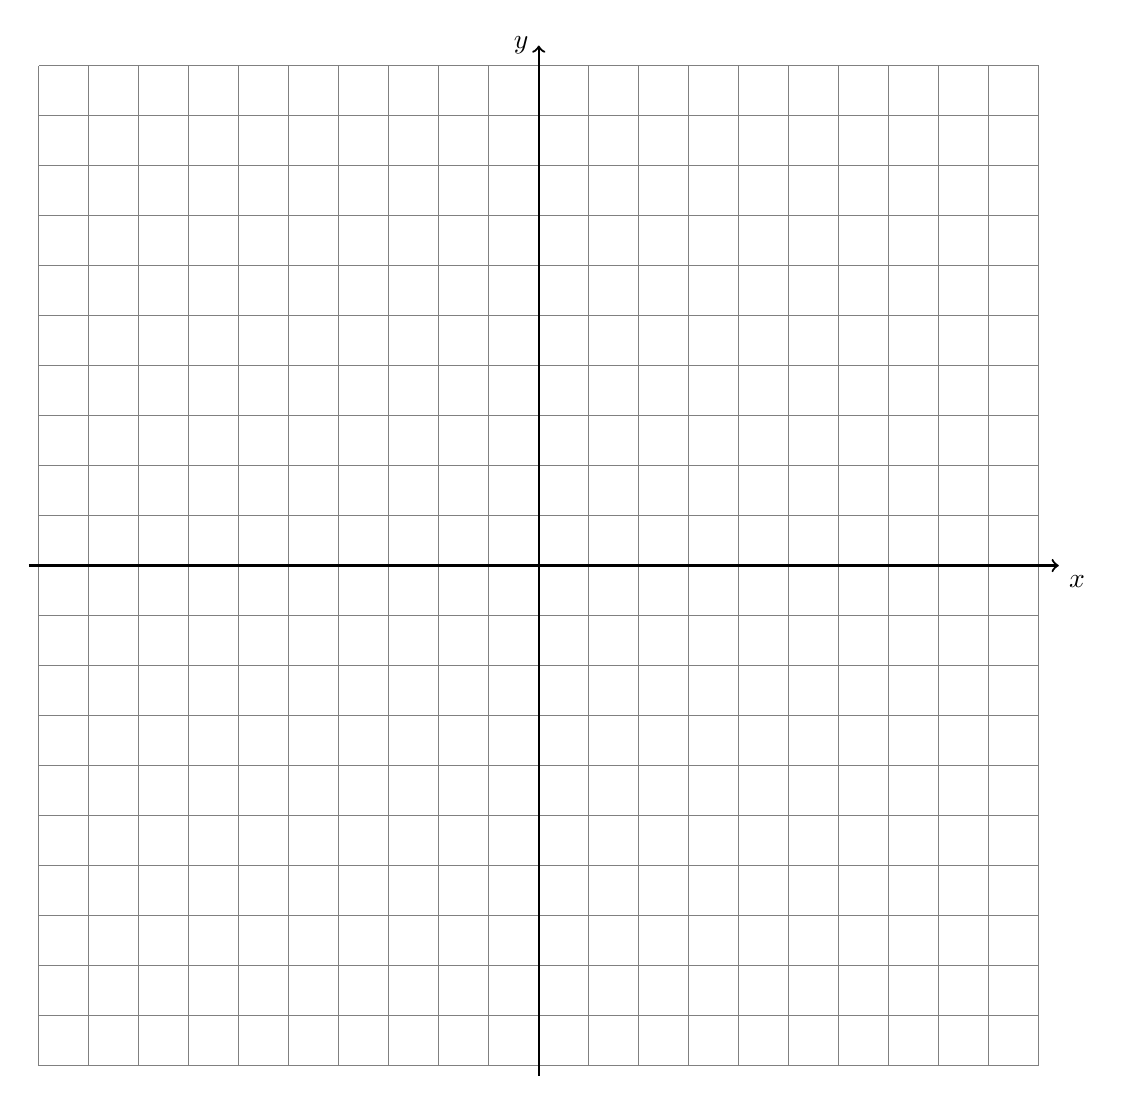
\begin{tikzpicture}[scale=.635]
      \draw [help lines] (-10,-10) grid (10,10);
      \draw [thick, ->] (-10.2,0) -- (10.4,0) node [below right] {$x$};
      \draw [thick, ->] (0,-10.2)--(0,10.4) node [left] {$y$};
    \end{tikzpicture}
    \end{center}
  Are the lines parallel, perpendicular, or neither? Justify your answer, stating the values of the lines' slopes.

\newpage
\item Given $J(-2,7)$ and $K(1,4)$, find the length of $\overline{JK}$. Leave the result in simplified radical form (not a decimal).
    \vspace{4cm}

\item On the graph below, draw $\overline{AB}$, with $A(-2,1)$ and $B(4,4)$, labeling the end points.\\
  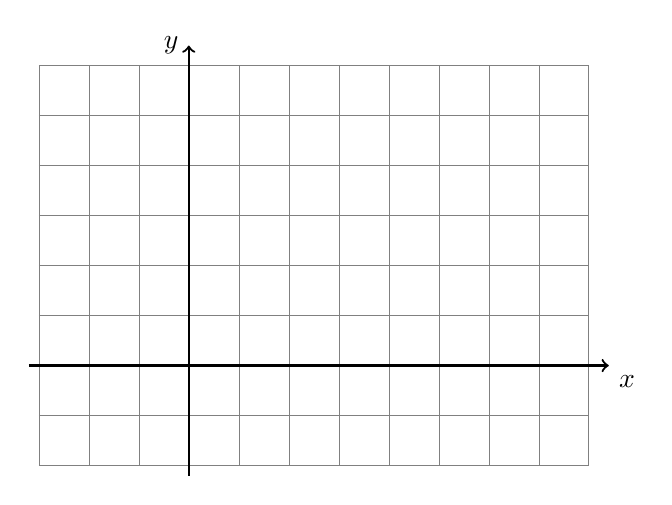
\begin{tikzpicture}[scale=.635]
    \draw [help lines] (-3,-2) grid (8,6);
    \draw [thick, ->] (-3.2,0) -- (8.4,0) node [below right] {$x$};
    \draw [thick, ->] (0,-2.2)--(0,6.4) node [left] {$y$};
  \end{tikzpicture}
  \begin{enumerate}
    \item Determine and state the coordinates of the midpoint $M$ of $\overline{AB}$. Mark $M$ and label it on the graph. \vspace{2cm}
    \item Find the slope of $\overline{AB}$. \vspace{2.5cm}
    \item Find the length of $\overline{AB}$. Leave the result as a simplified radical.
  \end{enumerate}

\newpage
\item In the diagram below, $\overline{AC}$ has endpoints with coordinates $A(-3,-3)$ and $C(7, 2)$.
  \begin{center} %4 quadrant regents grid
    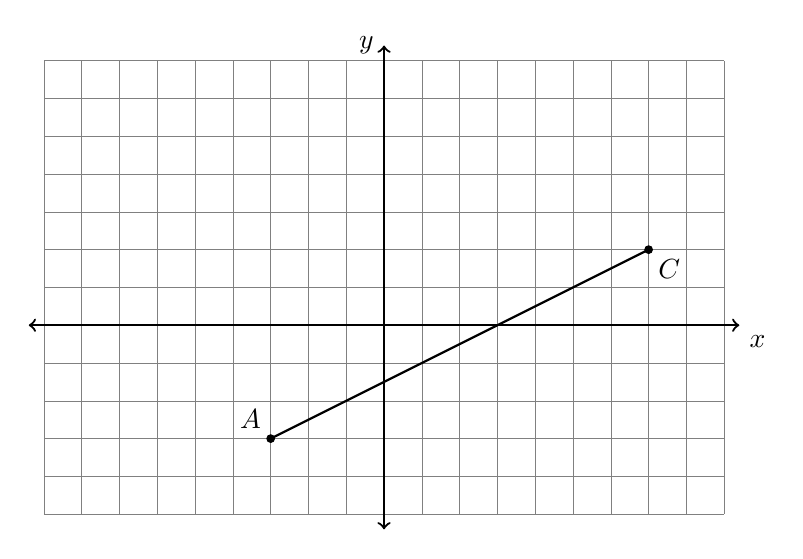
\begin{tikzpicture}[scale=.48]
      \draw [help lines] (-9,-5) grid (9,7);
      \draw [thick, <->] (-9.4,0) -- (9.4,0) node [below right] {$x$};
      \draw [thick, <->] (0,-5.4)--(0,7.4) node [left] {$y$};
      \draw [thick] (-3,-3)--(7, 2);
      \draw [fill] (-3,-3) circle [radius=0.1] node[above left] {$A$};
      \draw [fill] (7, 2) circle [radius=0.1] node[below right] {$C$};
    \end{tikzpicture}
  \end{center}
  If $B$ is a point on $\overline{AC}$ and $AB {:} BC = 2{:}3$,  what  are  the coordinates of $B$? \vspace{4cm}

  \item $A(2,4)$ is one endpoint of $\overline{AB}$. The segment's midpoint is $M(7,3)$. Find the other endpoint, $B$. \vspace{3cm}

  \item A translation maps $A(-1,12) \rightarrow A'(5,6)$. What is the image of $B(10,-1)$ under the same translation?  \vspace{3cm}

\end{enumerate}
\end{document}
